\documentclass[11pt,a4paper]{article}
\usepackage[margin=0.72in]{geometry}
\usepackage[T1]{fontenc}
\usepackage{lmodern}
\usepackage{microtype}
\usepackage{amsmath,amssymb,mathtools}
\usepackage{array,booktabs,longtable,multicol}
\usepackage{xcolor}
\usepackage{enumitem}
\usepackage{tikz}
\usetikzlibrary{arrows.meta,calc,positioning,patterns}
\usepackage{fancyhdr}
\usepackage{titlesec}
\usepackage{hyperref}
\hypersetup{colorlinks=true,linkcolor=blue!50!black,urlcolor=blue!50!black}

\definecolor{headblue}{HTML}{12355B}
\definecolor{lightblue}{HTML}{EAF3FF}
\definecolor{ansgreen}{HTML}{0B6B3A}
\definecolor{softgray}{HTML}{F5F7FA}

\pagestyle{fancy}
\fancyhf{}
\lhead{BCS-012 Basic Mathematics}
\rhead{Solved Paper: June 2024}
\cfoot{\thepage}
\renewcommand{\headrulewidth}{0.4pt}
\setlength{\headheight}{14pt}

\titleformat{\section}{\Large\bfseries\color{headblue}}{}{0pt}{}
\titleformat{\subsection}{\large\bfseries\color{headblue}}{}{0pt}{}
\setlist[itemize]{leftmargin=*,itemsep=2pt,topsep=2pt}
\setlist[enumerate]{leftmargin=*,itemsep=2pt,topsep=2pt}
\setlength{\parindent}{0pt}
\setlength{\parskip}{5pt}

\newcommand{\qpart}[2]{\subsection*{#1 \hfill {\normalsize[#2 marks]}}}
\newcommand{\answer}{\textbf{Answer.} }
\newcommand{\finalans}[1]{\par\noindent\fcolorbox{ansgreen}{green!4}{\parbox{0.96\linewidth}{\textbf{Final answer:} #1}}}
\newcommand{\note}[1]{\par\noindent\fcolorbox{orange!70!black}{orange!8}{\parbox{0.96\linewidth}{\textbf{Note:} #1}}}

\begin{document}

\begin{center}
{\LARGE\bfseries IGNOU BCS-012: Basic Mathematics}\\[2mm]
{\Large\bfseries Term-End Examination, June 2024 - Fully Solved}\\[1mm]
{\normalsize BCA (Revised) \quad Time: 3 Hours \quad Maximum Marks: 100}\\[2mm]
\rule{0.88\linewidth}{0.5pt}
\end{center}

\tableofcontents
\newpage

\section*{Question 1}
\addcontentsline{toc}{section}{Question 1}

\qpart{1(a) Show that}{5}
\[
\begin{vmatrix}
b+c&c+a&a+b\\
c+a&a+b&b+c\\
a+b&b+c&c+a
\end{vmatrix}
=2\begin{vmatrix}
a&b&c\\ b&c&a\\ c&a&b
\end{vmatrix}.
\]
\answer Let $s=a+b+c$ and
\[
N=\begin{pmatrix}a&b&c\\ b&c&a\\ c&a&b\end{pmatrix},\qquad
J=\begin{pmatrix}1&1&1\\1&1&1\\1&1&1\end{pmatrix}.
\]
The matrix on the left is
\[
M=\begin{pmatrix}s-a&s-b&s-c\\s-b&s-c&s-a\\s-c&s-a&s-b\end{pmatrix}=sJ-N.
\]
The vector $(1,1,1)^T$ is an eigenvector of $N$ with eigenvalue $s$. Therefore for $M=sJ-N$, the eigenvalue of $J$ on $(1,1,1)^T$ is $3$, so the eigenvalue of $M$ on this vector is $3s-s=2s$. On the two-dimensional subspace $x+y+z=0$, $J$ acts as zero, so $M=-N$ there. Hence the three eigenvalues of $M$ are $2s,-\lambda_2,-\lambda_3$, while those of $N$ are $s,\lambda_2,\lambda_3$. Thus
\[
\det M=(2s)(-\lambda_2)(-\lambda_3)=2s\lambda_2\lambda_3=2\det N.
\]
\finalans{The determinant identity is proved.}

\qpart{1(b) If $X=\begin{bmatrix}1&-2\\2&1\end{bmatrix}$ and $I_2=\begin{bmatrix}1&0\\0&1\end{bmatrix}$, find $(X-I_2)^2$}{5}
\answer
\[
X-I_2=\begin{bmatrix}0&-2\\2&0\end{bmatrix}.
\]
Therefore
\[
(X-I_2)^2=\begin{bmatrix}0&-2\\2&0\end{bmatrix}
\begin{bmatrix}0&-2\\2&0\end{bmatrix}
=\begin{bmatrix}-4&0\\0&-4\end{bmatrix}=-4I_2.
\]
\finalans{$(X-I_2)^2=\begin{bmatrix}-4&0\\0&-4\end{bmatrix}$.}

\qpart{1(c) Find the sum up to $n$ terms of $0.3+0.33+0.333+\cdots$}{5}
\answer The $r$th term is
\[
0.\underbrace{33\cdots3}_{r\text{ times}}=3\left(10^{-1}+10^{-2}+\cdots+10^{-r}\right)=\frac13(1-10^{-r}).
\]
Thus
\[
S_n=\sum_{r=1}^{n}\frac13(1-10^{-r})
=\frac n3-\frac13\sum_{r=1}^{n}10^{-r}.
\]
Now
\[
\sum_{r=1}^{n}10^{-r}=\frac{1}{10}\frac{1-10^{-n}}{1-\frac1{10}}=\frac19(1-10^{-n}).
\]
Hence
\[
S_n=\frac n3-\frac1{27}(1-10^{-n}).
\]
\finalans{$S_n=\dfrac n3-\dfrac1{27}(1-10^{-n})$.}

\qpart{1(d) If 7 times the 7th term of an A.P. is equal to 11 times the 11th term, find the 18th term}{5}
\answer Let the A.P. have first term $a$ and common difference $d$. Then $T_r=a+(r-1)d$.
\[
7T_7=11T_{11}
\Rightarrow 7(a+6d)=11(a+10d).
\]
So
\[
7a+42d=11a+110d \Rightarrow 4a+68d=0 \Rightarrow a=-17d.
\]
The 18th term is
\[
T_{18}=a+17d=-17d+17d=0.
\]
\finalans{$T_{18}=0$.}

\qpart{1(e) If $1,\omega,\omega^2$ are cube roots of unity, find $(2+\omega+\omega^2)^6+(3+\omega+\omega^2)^6$}{5}
\answer For cube roots of unity,
\[
1+\omega+\omega^2=0 \Rightarrow \omega+\omega^2=-1.
\]
Therefore
\[
2+\omega+\omega^2=1,\qquad 3+\omega+\omega^2=2.
\]
Hence
\[
(2+\omega+\omega^2)^6+(3+\omega+\omega^2)^6=1^6+2^6=1+64=65.
\]
\finalans{$65$.}

\qpart{1(f) Find the quadratic equation with real coefficients and roots $\dfrac{m-n}{m+n},-\dfrac{m+n}{m-n}$}{5}
\answer Let
\[
\alpha=\frac{m-n}{m+n},\qquad \beta=-\frac{m+n}{m-n}.
\]
Then
\[
\alpha\beta=-1.
\]
Also
\[
\alpha+\beta=\frac{m-n}{m+n}-\frac{m+n}{m-n}
=\frac{(m-n)^2-(m+n)^2}{m^2-n^2}
=\frac{-4mn}{m^2-n^2}.
\]
The required equation is
\[
x^2-(\alpha+\beta)x+\alpha\beta=0.
\]
Thus
\[
x^2+\frac{4mn}{m^2-n^2}x-1=0.
\]
Multiplying by $m^2-n^2$,
\[
(m^2-n^2)x^2+4mnx-(m^2-n^2)=0.
\]
\finalans{$(m^2-n^2)x^2+4mnx-(m^2-n^2)=0$.}

\qpart{1(g) Evaluate $\int x\sqrt{3-2x}\,dx$}{5}
\answer Put $u=3-2x$. Then $du=-2dx$, $dx=-du/2$, and $x=(3-u)/2$.
\[
\int x\sqrt{3-2x}\,dx
=-\frac14\int (3-u)u^{1/2}\,du.
\]
So
\[
=-\frac14\left(3\cdot\frac{2}{3}u^{3/2}-\frac{2}{5}u^{5/2}\right)+C
=-\frac12u^{3/2}+\frac1{10}u^{5/2}+C.
\]
Substituting $u=3-2x$,
\[
\int x\sqrt{3-2x}\,dx=\frac1{10}(3-2x)^{5/2}-\frac12(3-2x)^{3/2}+C.
\]
Equivalently,
\[
=-\frac{x+1}{5}(3-2x)^{3/2}+C.
\]
\finalans{$\displaystyle -\frac{x+1}{5}(3-2x)^{3/2}+C$.}

\qpart{1(h) A spherical balloon is inflated at $900\,\text{cm}^3/\text{s}$. How fast is radius increasing when $r=25\,\text{cm}$?}{5}
\answer For a sphere,
\[
V=\frac43\pi r^3.
\]
Differentiating with respect to $t$,
\[
\frac{dV}{dt}=4\pi r^2\frac{dr}{dt}.
\]
Given $dV/dt=900$ and $r=25$,
\[
900=4\pi(25)^2\frac{dr}{dt}=2500\pi\frac{dr}{dt}.
\]
Thus
\[
\frac{dr}{dt}=\frac{900}{2500\pi}=\frac{9}{25\pi}\,\text{cm/s}.
\]
\finalans{$\displaystyle \frac{dr}{dt}=\frac{9}{25\pi}\,\text{cm/s}\approx0.115\,\text{cm/s}$.}

\newpage
\section*{Question 2}
\addcontentsline{toc}{section}{Question 2}

\qpart{2(a) Solve by matrix method}{5}
\[
2x-y+3z=5,\qquad 3x+2y-z=7,
\qquad 4x+5y-5z=9.
\]
\answer The augmented matrix is
\[
\left[\begin{array}{ccc|c}
2&-1&3&5\\
3&2&-1&7\\
4&5&-5&9
\end{array}\right].
\]
Solving the linear system by row reduction gives
\[
x=\frac{43}{18},\qquad y=-\frac1{18},\qquad z=\frac1{18}.
\]
Verification:
\[
2\left(\frac{43}{18}\right)-\left(-\frac1{18}\right)+3\left(\frac1{18}\right)=\frac{86+1+3}{18}=5,
\]
\[
3\left(\frac{43}{18}\right)+2\left(-\frac1{18}\right)-\frac1{18}=\frac{129-2-1}{18}=7,
\]
\[
4\left(\frac{43}{18}\right)+5\left(-\frac1{18}\right)-5\left(\frac1{18}\right)=\frac{172-5-5}{18}=9.
\]
\finalans{$x=\dfrac{43}{18},\ y=-\dfrac1{18},\ z=\dfrac1{18}$.}

\qpart{2(b) Use mathematical induction to show $1+4+7+\cdots+(3n-2)=\frac12 n(3n-1)$}{5}
\answer Let
\[
P(n):\quad 1+4+7+\cdots+(3n-2)=\frac12n(3n-1).
\]
For $n=1$,
\[
\text{LHS}=1,
\qquad \text{RHS}=\frac12(1)(3-1)=1.
\]
So $P(1)$ is true.

Assume $P(k)$ is true:
\[
1+4+\cdots+(3k-2)=\frac12k(3k-1).
\]
For $k+1$,
\[
1+4+\cdots+(3k-2)+[3(k+1)-2]
=\frac12k(3k-1)+(3k+1).
\]
\[
=\frac{3k^2-k+6k+2}{2}
=\frac{3k^2+5k+2}{2}
=\frac{(k+1)(3k+2)}{2}.
\]
But
\[
\frac12(k+1)(3(k+1)-1)=\frac12(k+1)(3k+2).
\]
Thus $P(k+1)$ is true. Hence, by induction, the formula holds for all $n\in\mathbb N$.
\finalans{The identity is proved by mathematical induction.}

\qpart{2(c) Find quadratic equation with roots $\dfrac1{5-\sqrt{72}},\dfrac1{5+6\sqrt2}$}{5}
\answer Since $\sqrt{72}=6\sqrt2$, the roots are
\[
\alpha=\frac1{5-6\sqrt2},\qquad \beta=\frac1{5+6\sqrt2}.
\]
Then
\[
\alpha+\beta=\frac{(5+6\sqrt2)+(5-6\sqrt2)}{25-72}=\frac{10}{-47}=-\frac{10}{47},
\]
\[
\alpha\beta=\frac1{(5-6\sqrt2)(5+6\sqrt2)}=\frac1{25-72}=-\frac1{47}.
\]
The equation is
\[
x^2-(\alpha+\beta)x+\alpha\beta=0.
\]
Therefore
\[
x^2+\frac{10}{47}x-\frac1{47}=0.
\]
Multiplying by 47,
\[
47x^2+10x-1=0.
\]
\finalans{$47x^2+10x-1=0$.}

\qpart{2(d) If $\left(\dfrac{1-i}{1+i}\right)^{10}=a+ib$, show the values of $a$ and $b$}{5}
\answer First simplify the base:
\[
\frac{1-i}{1+i}=\frac{(1-i)^2}{(1+i)(1-i)}
=\frac{1-2i+i^2}{2}=\frac{-2i}{2}=-i.
\]
Thus
\[
\left(\frac{1-i}{1+i}\right)^{10}=(-i)^{10}=(((-i)^4\bigr)^2(-i)^2=1^2(-1)=-1.
\]
Hence
\[
a+ib=-1+0i.
\]
\note{The printed question says to show $a=1$ and $b=0$, but direct calculation gives $a=-1$ and $b=0$. Therefore the printed statement appears to contain a sign or exponent error.}
\finalans{$a=-1,\ b=0$ for the expression as printed.}

\newpage
\section*{Question 3}
\addcontentsline{toc}{section}{Question 3}

\qpart{3(a) If $A=\begin{bmatrix}1&1&3\\0&5&2\\2&-1&7\end{bmatrix}$, show that $A$ is row equivalent to $I_3$}{5}
\answer A square matrix is row equivalent to $I_3$ if its determinant is non-zero. Here
\[
\det A=
\begin{vmatrix}
1&1&3\\0&5&2\\2&-1&7
\end{vmatrix}.
\]
Expanding along the first row,
\[
\det A=1(35+2)-1(0-4)+3(0-10)
=37+4-30=11.
\]
Since $\det A=11\ne0$, $A$ is non-singular. Hence it can be reduced by elementary row operations to the identity matrix $I_3$.
\[
A\sim I_3.
\]
\finalans{$A$ is row equivalent to $I_3$ because $\det A=11\ne0$.}

\qpart{3(b) Solve $\dfrac{2x-5}{x+2}<5$, $x\in\mathbb R$, and graph the solution set}{5}
\answer The expression is not defined at $x=-2$.
\[
\frac{2x-5}{x+2}<5
\Rightarrow \frac{2x-5-5x-10}{x+2}<0
\Rightarrow \frac{-3x-15}{x+2}<0.
\]
\[
\Rightarrow -3\frac{x+5}{x+2}<0
\Rightarrow \frac{x+5}{x+2}>0.
\]
Critical points are $x=-5$ and $x=-2$. Testing intervals gives
\[
(-\infty,-5): +,\qquad (-5,-2): -,\qquad (-2,\infty): +.
\]
Therefore
\[
x\in(-\infty,-5)\cup(-2,\infty).
\]
\begin{center}
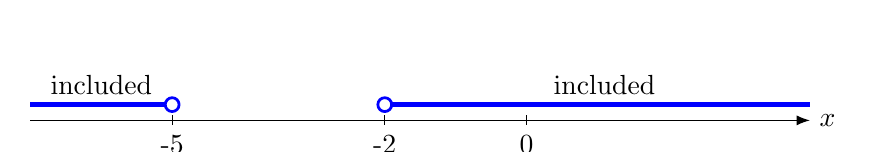
\begin{tikzpicture}[x=0.9cm,y=0.8cm]
\draw[-Latex] (-7,0)--(4,0) node[right]{$x$};
\foreach \x/\lab in {-5/-5,-2/-2,0/0} {\draw (\x,0.08)--(\x,-0.08) node[below]{\lab};}
\draw[line width=2pt,blue] (-7,0.25)--(-5,0.25);
\draw[line width=2pt,blue] (-2,0.25)--(4,0.25);
\draw[fill=white,draw=blue,line width=1pt] (-5,0.25) circle (2.5pt);
\draw[fill=white,draw=blue,line width=1pt] (-2,0.25) circle (2.5pt);
\node[above] at (-6,0.25){included};
\node[above] at (1.1,0.25){included};
\end{tikzpicture}
\end{center}
\finalans{$(-\infty,-5)\cup(-2,\infty)$.}

\qpart{3(c) Solve $32x^3-48x^2+22x-3=0$, given roots are in A.P.}{5}
\answer Factorising the polynomial,
\[
32x^3-48x^2+22x-3=(2x-1)(4x-1)(4x-3).
\]
Therefore,
\[
2x-1=0\Rightarrow x=\frac12,
\]
\[
4x-1=0\Rightarrow x=\frac14,
\]
\[
4x-3=0\Rightarrow x=\frac34.
\]
The roots are
\[
\frac14,\frac12,\frac34,
\]
which are in A.P. with common difference $\frac14$.
\finalans{$x=\dfrac14,\dfrac12,\dfrac34$.}

\qpart{3(d) Determine the local maxima and local minima of $f(x)=x^3-6x^2+9x+100$}{5}
\answer
\[
f'(x)=3x^2-12x+9=3(x-1)(x-3).
\]
Critical points are $x=1$ and $x=3$.
\[
f''(x)=6x-12.
\]
At $x=1$,
\[
f''(1)=6-12=-6<0,
\]
so $x=1$ gives local maximum.
\[
f(1)=1-6+9+100=104.
\]
At $x=3$,
\[
f''(3)=18-12=6>0,
\]
so $x=3$ gives local minimum.
\[
f(3)=27-54+27+100=100.
\]
\finalans{Local maximum: $(1,104)$. Local minimum: $(3,100)$.}

\newpage
\section*{Question 4}
\addcontentsline{toc}{section}{Question 4}

\qpart{4(a) Check continuity at $x=0$ for $f(x)=\begin{cases} \dfrac{2|x|}{x},&x\ne0,\\0,&x=0.\end{cases}$}{5}
\answer For $x>0$, $|x|=x$, so
\[
f(x)=\frac{2x}{x}=2.
\]
Thus
\[
\lim_{x\to0^+}f(x)=2.
\]
For $x<0$, $|x|=-x$, so
\[
f(x)=\frac{2(-x)}{x}=-2.
\]
Thus
\[
\lim_{x\to0^-}f(x)=-2.
\]
Since the left-hand and right-hand limits are not equal, $\lim_{x\to0}f(x)$ does not exist. Also $f(0)=0$.
\finalans{$f(x)$ is not continuous at $x=0$.}

\qpart{4(b) Find vector and cartesian equations of the line through $(1,-1,-2)$ and parallel to $3\hat i-2\hat j+5\hat k$}{5}
\answer The point is $(1,-1,-2)$ and the direction vector is $(3,-2,5)$.

The vector equation is
\[
\vec r=(\hat i-\hat j-2\hat k)+\lambda(3\hat i-2\hat j+5\hat k),\qquad \lambda\in\mathbb R.
\]
The parametric equations are
\[
x=1+3\lambda,
\qquad y=-1-2\lambda,
\qquad z=-2+5\lambda.
\]
Hence the cartesian equation is
\[
\frac{x-1}{3}=\frac{y+1}{-2}=\frac{z+2}{5}.
\]
\finalans{$\vec r=(\hat i-\hat j-2\hat k)+\lambda(3\hat i-2\hat j+5\hat k)$ and $\dfrac{x-1}{3}=\dfrac{y+1}{-2}=\dfrac{z+2}{5}$.}

\qpart{4(c) Determine the length of the curve $y=2x^{3/2}$ from $(1,2)$ to $(4,16)$}{5}
\answer The arc length is
\[
L=\int_a^b \sqrt{1+\left(\frac{dy}{dx}\right)^2}\,dx.
\]
Given
\[
y=2x^{3/2}\Rightarrow \frac{dy}{dx}=3x^{1/2}=3\sqrt{x}.
\]
Therefore
\[
L=\int_1^4\sqrt{1+9x}\,dx.
\]
Let $u=1+9x$, so $du=9dx$.
\[
L=\frac19\int_{10}^{37}u^{1/2}\,du
=\frac19\left[\frac23u^{3/2}\right]_{10}^{37}
=\frac{2}{27}\left(37^{3/2}-10^{3/2}\right).
\]
\finalans{$\displaystyle L=\frac{2}{27}\left(37^{3/2}-10^{3/2}\right)$.}

\qpart{4(d) Find the sum of all integers between 100 and 1000 divisible by 9}{5}
\answer The first multiple of 9 greater than 100 is $108$ and the last multiple of 9 less than 1000 is $999$.

This is an A.P.:
\[
108,117,126,\ldots,999
\]
with $a=108$, $d=9$, and $l=999$.
\[
l=a+(n-1)d
\Rightarrow 999=108+(n-1)9.
\]
\[
891=9(n-1)\Rightarrow n-1=99\Rightarrow n=100.
\]
Sum is
\[
S_n=\frac n2(a+l)=\frac{100}{2}(108+999)=50\times1107=55350.
\]
\finalans{$55350$.}

\newpage
\section*{Question 5}
\addcontentsline{toc}{section}{Question 5}

\qpart{5(a) Maximize $5x+2y$ subject to the given constraints}{5}
\[
-2x-3y\le -6,\quad x-2y\le2,
\quad 6x+4y\le24,
\quad -3x+2y\le3,
\quad x\ge0,\ y\ge0.
\]
\answer Convert the first and third constraints:
\[
2x+3y\ge6,
\qquad 3x+2y\le12.
\]
The boundary lines are
\[
2x+3y=6,
\quad x-2y=2,
\quad 3x+2y=12,
\quad -3x+2y=3.
\]
The feasible corner points are obtained by intersecting boundary lines:
\[
\left(\frac{18}{7},\frac{2}{7}\right),
\quad \left(\frac{3}{13},\frac{24}{13}\right),
\quad \left(\frac72,\frac34\right),
\quad \left(\frac32,\frac{15}{4}\right).
\]
Evaluate $Z=5x+2y$:
\[
\begin{array}{c|c}
\text{Corner point} & Z=5x+2y\\ \hline
\left(\frac{18}{7},\frac{2}{7}\right)&\frac{94}{7}\\
\left(\frac{3}{13},\frac{24}{13}\right)&\frac{63}{13}\\
\left(\frac72,\frac34\right)&19\\
\left(\frac32,\frac{15}{4}\right)&15
\end{array}
\]
The maximum is $19$ at $\left(\frac72,\frac34\right)$.

\begin{center}
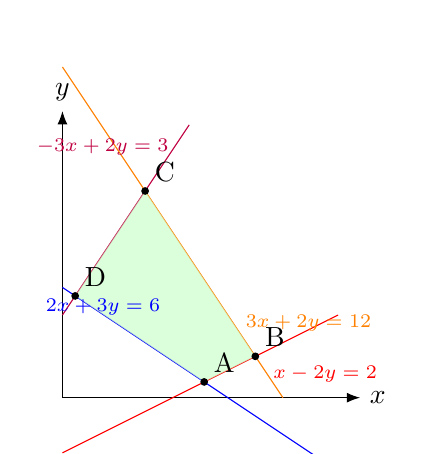
\begin{tikzpicture}[scale=0.7]
\draw[-Latex] (0,0)--(5.4,0) node[right]{$x$};
\draw[-Latex] (0,0)--(0,5.2) node[above]{$y$};
\draw[domain=0:4.8,smooth,variable=\x,blue] plot ({\x},{(6-2*\x)/3});
\draw[domain=0:5,smooth,variable=\x,red] plot ({\x},{(\x-2)/2});
\draw[domain=0:4,smooth,variable=\x,orange] plot ({\x},{(12-3*\x)/2});
\draw[domain=0:2.3,smooth,variable=\x,purple] plot ({\x},{(3+3*\x)/2});
\fill[green!20,opacity=0.7] (18/7,2/7)--(7/2,3/4)--(3/2,15/4)--(3/13,24/13)--cycle;
\fill (18/7,2/7) circle (2pt) node[above right]{A};
\fill (7/2,3/4) circle (2pt) node[above right]{B};
\fill (3/2,15/4) circle (2pt) node[above right]{C};
\fill (3/13,24/13) circle (2pt) node[above right]{D};
\node[blue,anchor=east,font=\scriptsize] at (1.95,1.65){$2x+3y=6$};
\node[red,anchor=west,font=\scriptsize] at (3.65,0.42){$x-2y=2$};
\node[orange,anchor=west,font=\scriptsize] at (3.15,1.35){$3x+2y=12$};
\node[purple,anchor=east,font=\scriptsize] at (2.1,4.55){$-3x+2y=3$};
\end{tikzpicture}
\end{center}
\finalans{Maximum value is $19$ at $\left(\dfrac72,\dfrac34\right)$.}

\qpart{5(b) Find the area bounded by $y=x^2$ and $y^2=x$}{5}
\answer The curve $y^2=x$ gives $y=\sqrt{x}$ for the upper branch in the first quadrant. Intersections satisfy
\[
y=x^2,
\qquad x=y^2.
\]
Substitute $x=y^2$ into $y=x^2$:
\[
y=(y^2)^2=y^4
\Rightarrow y(y^3-1)=0.
\]
So $y=0,1$, giving intersection points $(0,0)$ and $(1,1)$.

For $0\le x\le1$, upper curve is $y=\sqrt{x}$ and lower curve is $y=x^2$. Therefore area is
\[
A=\int_0^1(\sqrt{x}-x^2)\,dx.
\]
\[
A=\left[\frac23x^{3/2}-\frac13x^3\right]_0^1
=\frac23-\frac13=\frac13.
\]
\begin{center}
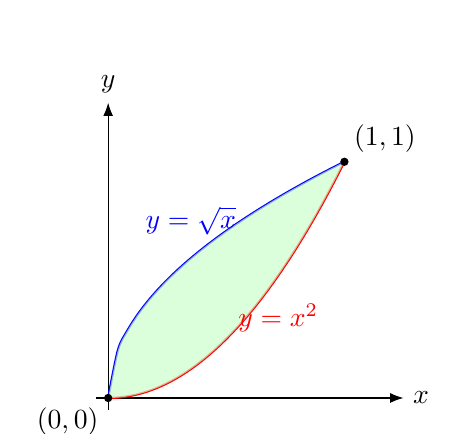
\begin{tikzpicture}[scale=3]
\draw[-Latex] (-0.05,0)--(1.25,0) node[right]{$x$};
\draw[-Latex] (0,-0.05)--(0,1.25) node[above]{$y$};
\draw[domain=0:1,smooth,variable=\x,blue,thick] plot ({\x},{sqrt(\x)});
\draw[domain=0:1,smooth,variable=\x,red,thick] plot ({\x},{\x*\x});
\fill[green!20,opacity=0.7] plot[domain=0:1,smooth] (\x,{sqrt(\x)}) -- plot[domain=1:0,smooth] (\x,{\x*\x}) -- cycle;
\node[blue] at (0.35,0.75){$y=\sqrt{x}$};
\node[red] at (0.72,0.34){$y=x^2$};
\fill (0,0) circle (0.5pt) node[below left]{$(0,0)$};
\fill (1,1) circle (0.5pt) node[above right]{$(1,1)$};
\end{tikzpicture}
\end{center}
\finalans{Area $=\dfrac13$ square unit.}

\qpart{5(c) Reduce $A=\begin{bmatrix}0&1&2\\1&2&3\\3&1&1\end{bmatrix}$ to normal form and determine rank}{5}
\answer The determinant is
\[
\det A=\begin{vmatrix}0&1&2\\1&2&3\\3&1&1\end{vmatrix}.
\]
Expanding along the first row,
\[
\det A= -1\begin{vmatrix}1&3\\3&1\end{vmatrix}
+2\begin{vmatrix}1&2\\3&1\end{vmatrix}
=-(1-9)+2(1-6)=8-10=-2.
\]
Since $\det A=-2\ne0$, the matrix is non-singular and row-column equivalent to $I_3$.
Thus its normal form is
\[
\begin{bmatrix}1&0&0\\0&1&0\\0&0&1\end{bmatrix}.
\]
Hence the rank is $3$.
\finalans{Normal form $=I_3$ and $\operatorname{rank}(A)=3$.}

\qpart{5(d) If $\vec a+\vec b+\vec c=\vec0$, show that $\vec a\times\vec b=\vec b\times\vec c=\vec c\times\vec a$}{5}
\answer Given
\[
\vec a+\vec b+\vec c=\vec0.
\]
So
\[
\vec c=-(\vec a+\vec b).
\]
Now
\[
\vec b\times\vec c=\vec b\times[-(\vec a+\vec b)]
=-\vec b\times\vec a-\vec b\times\vec b.
\]
Since $\vec b\times\vec b=\vec0$ and $\vec b\times\vec a=-\vec a\times\vec b$,
\[
\vec b\times\vec c=\vec a\times\vec b.
\]
Also
\[
\vec c\times\vec a=[-(\vec a+\vec b)]\times\vec a
=-\vec a\times\vec a-\vec b\times\vec a
=\vec a\times\vec b.
\]
Therefore
\[
\vec a\times\vec b=\vec b\times\vec c=\vec c\times\vec a.
\]
\finalans{The required vector product identity is proved.}

\newpage
\section*{Last Page: Theory and Formula Sheet}
\addcontentsline{toc}{section}{Last Page: Theory and Formula Sheet}
\small
\begin{multicols}{2}
\textbf{Determinants and matrices.}
For a square matrix $A$, if $\det A\ne0$, then $A$ is non-singular and row equivalent to $I$. A quadratic equation with roots $\alpha,\beta$ is $x^2-(\alpha+\beta)x+\alpha\beta=0$. For matrix powers, first simplify the matrix expression and then multiply.

\textbf{A.P. and series.}
The $n$th term of an A.P. is $T_n=a+(n-1)d$. The sum of an A.P. is $S_n=\frac n2[2a+(n-1)d]=\frac n2(a+l)$. For a finite G.P., $a+ar+\cdots+ar^{n-1}=a\frac{1-r^n}{1-r}$.

\textbf{Complex numbers.}
For cube roots of unity, $1+\omega+\omega^2=0$ and $\omega^3=1$. Also $i^2=-1$, $i^4=1$. Rationalize complex fractions by multiplying numerator and denominator by the conjugate.

\textbf{Calculus.}
For integration by substitution, put the inner expression equal to $u$. Related rates use differentiation with respect to time. For a sphere, $V=\frac43\pi r^3$ and $\frac{dV}{dt}=4\pi r^2\frac{dr}{dt}$. Arc length is $L=\int_a^b\sqrt{1+(dy/dx)^2}\,dx$.

\textbf{Continuity and extrema.}
A function is continuous at $a$ if $\lim_{x\to a^-}f(x)=\lim_{x\to a^+}f(x)=f(a)$. For local maxima/minima, solve $f'(x)=0$. If $f''(a)<0$, local maximum; if $f''(a)>0$, local minimum.

\textbf{Induction.}
To prove $P(n)$: prove $P(1)$, assume $P(k)$, then prove $P(k+1)$. This proves the result for all $n\in\mathbb N$.

\textbf{Inequalities.}
Move all terms to one side, factor, identify critical points, and use a sign chart. Denominator zeros are excluded from the solution set.

\textbf{Coordinate geometry and vectors.}
Line through point $\vec r_0$ parallel to vector $\vec v$ is $\vec r=\vec r_0+\lambda\vec v$. Cartesian form: $\frac{x-x_1}{a}=\frac{y-y_1}{b}=\frac{z-z_1}{c}$. If $\vec a+\vec b+\vec c=0$, then substitute one vector as negative sum of the other two.

\textbf{Linear programming.}
Convert each inequality into a boundary line. Find the feasible region, calculate all corner points, and evaluate the objective function at each corner. Maximum/minimum occurs at a corner point for a bounded feasible polygon.

\textbf{Area between curves.}
Area is $\int(\text{upper curve}-\text{lower curve})dx$ or $\int(\text{right curve}-\text{left curve})dy$ after finding intersection limits.
\end{multicols}

\end{document}
